\documentclass[10pt]{article}
\usepackage[T1]{fontenc}
\usepackage[tt=false]{libertine}
\usepackage[varqu]{zi4}
\usepackage[a4paper,margin=2.3cm]{geometry}
\usepackage{amsmath,amssymb}
\usepackage{booktabs}
\usepackage{tabularx}
\usepackage{xcolor}
\usepackage{listings}
\usepackage{tikz}
\usetikzlibrary{arrows.meta,positioning,calc,fit,backgrounds}
\usepackage{caption}
\usepackage[hidelinks]{hyperref}
\usepackage{enumitem}
\setlist{nosep,leftmargin=1.4em}
\setlength{\parskip}{0.35em}
\setlength{\parindent}{0pt}
\captionsetup{font=small,labelfont=bf}

% ---------------------------------------------------------------- listings
\lstdefinelanguage{sparql}{
  morekeywords={SELECT,WHERE,PREFIX,INSERT,DELETE,DATA,ORDER,BY,a},
  sensitive=true,
  morestring=[b]",
  morecomment=[l]{\#},
}
\lstdefinelanguage{nemo}{
  morekeywords={@parameter,@import,@export,@prefix},
  sensitive=true,
  morestring=[b]",
  morecomment=[l]{\%},
}
\lstset{
  basicstyle=\ttfamily\footnotesize,
  keywordstyle=\color{blue!60!black}\bfseries,
  stringstyle=\color{orange!60!black},
  commentstyle=\color{gray}\itshape,
  columns=fullflexible,
  keepspaces=true,
  frame=tb,
  framerule=0.4pt,
  aboveskip=6pt,
  belowskip=4pt,
  xleftmargin=2pt,
  breaklines=true,
  upquote=true,
  showstringspaces=false,
  literate={...}{{\textcolor{gray}{\dots}}}3,
}
\lstdefinestyle{py}{language=Python}
\lstdefinestyle{sq}{language=sparql}
\lstdefinestyle{nm}{language=nemo}

\newcommand{\brkunderscore}{\textunderscore\allowbreak}
\newcommand{\code}[1]{{\let\_\brkunderscore\texttt{#1}}}
\newcommand{\file}[1]{{\let\_\brkunderscore\texttt{#1}}}
\emergencystretch=3em

% ---------------------------------------------------------------- diagrams
\definecolor{pyfill}{HTML}{EAF2FB}
\definecolor{pyline}{HTML}{3B6EA8}
\definecolor{exfill}{HTML}{FDF1E3}
\definecolor{exline}{HTML}{B5701C}
\definecolor{crossc}{HTML}{B22222}
\definecolor{writec}{HTML}{C66A00}
\definecolor{tagS}{HTML}{8E44AD}
\definecolor{tagM}{HTML}{2E7D32}
\definecolor{tagP}{HTML}{00838F}

\tikzset{
  lane/.style={draw=#1, rounded corners=3pt, line width=0.7pt},
  lanelabel/.style={font=\footnotesize\bfseries, anchor=north west, inner sep=2pt},
  phasenode/.style={draw=black!70, rounded corners=2pt, fill=white, text width=2.05cm, align=center,
               minimum height=0.95cm, inner sep=2pt, font=\footnotesize},
  empty/.style={font=\footnotesize\itshape, text=black!55},
  flow/.style={-{Stealth[length=5pt,width=4pt]}, line width=0.6pt},
  call/.style={{Stealth[length=5pt,width=4pt]}-{Stealth[length=5pt,width=4pt]}, line width=0.6pt},
  cross/.style={-{Stealth[length=5pt,width=4pt]}, line width=1.1pt, draw=crossc},
  crosslabel/.style={font=\scriptsize, text=crossc, align=left, inner sep=1.5pt},
  head/.style={font=\footnotesize\bfseries, text=black!75},
  headswap/.style={head, text=crossc},
  badge/.style={font=\tiny\bfseries\sffamily, text=white, rounded corners=1pt, inner sep=1.4pt, fill=#1},
  rt/.style={circle, fill=crossc, text=white, font=\tiny\bfseries\sffamily, inner sep=0.8pt, minimum size=9pt},
  wr/.style={circle, fill=writec, text=white, font=\tiny\bfseries\sffamily, inner sep=0.8pt, minimum size=9pt},
}
% Column x positions of the six phases, lane geometry.
\def\cA{1.55}\def\cB{4.05}\def\cC{6.55}\def\cD{9.05}\def\cE{11.55}\def\cF{14.05}
\def\yP{0.85}\def\yX{-1.5}
% #1 = header names (six, comma separated) drawn above the columns
\newcommand{\headers}[6]{%
  \node[head] at (\cA,2.45) {#1}; \node[head] at (\cB,2.45) {#2}; \node[head] at (\cC,2.45) {#3};
  \node[head] at (\cD,2.45) {#4}; \node[head] at (\cE,2.45) {#5}; \node[head] at (\cF,2.45) {#6};}
\newcommand{\pylane}[1]{%
  \draw[lane=pyline, fill=pyfill] (0,0) rectangle (15.4,2.15);
  \node[lanelabel, text=pyline] at (0,2.15) {#1};}
\newcommand{\exlane}[2][solid]{%
  \draw[lane=exline, fill=exfill, #1] (0,-2.8) rectangle (15.4,-0.55);
  \node[lanelabel, text=exline, anchor=south west] at (0,-2.8) {#2};}
\newcommand{\nolane}[1]{%
  \draw[lane=black!35, dashed] (0,-2.8) rectangle (15.4,-0.55);
  \node[empty] at (7.7,-1.67) {#1};}
\newcommand{\tagS}[1]{\node[badge=tagS, anchor=south east] at ([xshift=-1pt,yshift=1pt]#1.north east) {S};}
\newcommand{\tagM}[1]{\node[badge=tagM, anchor=south east] at ([xshift=-1pt,yshift=1pt]#1.north east) {M};}
\newcommand{\tagP}[1]{\node[badge=tagP, anchor=south east] at ([xshift=-1pt,yshift=1pt]#1.north east) {P};}
\newcommand{\tagMP}[1]{\node[badge=tagP, anchor=south east] at ([xshift=-1pt,yshift=1pt]#1.north east) {P};
  \node[badge=tagM, anchor=south east] at ([xshift=-10pt,yshift=1pt]#1.north east) {M};}

\title{\textbf{The Agent Loop}\\[2pt]\large Supplementary description of the delivery-robot experiment (Section~7.4, Table~4)}
\date{}
\author{}

\begin{document}
\maketitle
\vspace{-3em}

\tableofcontents

% =====================================================================
\section{What the experiment asks}
\label{sec:question}

An agent that uses OWL knowledge rarely decides with logical inference alone. A delivery robot needs inferred facts
(who is a member of a college, who is a T20 cricket fan) and it needs its own procedures (can it reach a room with its
battery, how long does it take to drive there). These procedures read the robot's current state, which changes every
step. They are \emph{computables} in the sense of KnowRob: their values are computed when a query needs them, not
stored.

The experiment asks two questions.
\begin{enumerate}
  \item Can such an agent decide with \emph{one} world model, in which perception updates the knowledge, the OWL~2~RL
        consequences follow, and the decision query calls the planner directly?
  \item What does a \emph{second} world model cost: in code that synchronizes the two representations, in
        statements written per step, in requests to another process, and in time per step?
\end{enumerate}

To answer them, the same robot is built several ways. Everything except the knowledge layer is the same code in every
build:
\begin{itemize}
  \item \textbf{Scenario.} The campus map, the course rooms and mail boxes, the robot's start, and the perceptions of
        every step are generated once per seed from the raw OWL2Bench data, with RDFLib and without reasoning, and
        written to a file that every build reads (\file{scenario.py}). Seeds 0--4, 200 steps each.
  \item \textbf{Robot and planner.} The robot, its path planner (Dijkstra's algorithm on the map) and its two
        procedures \code{can\_reach} and \code{travel\_seconds} are one module (\file{robot.py}, \file{campus.py}).
  \item \textbf{Decisions.} The two decision queries ask the same question in every build (Section~\ref{sec:decisions}),
        and the policy that picks the action from their answers is one class, \code{DeliveryPolicy}.
  \item \textbf{States.} Every build except the reference (KRROOD) carries out the reference's action in every step,
        not its own. All builds therefore see the same robot states. Each build's own decision and its candidate sets
        are still recorded and compared with the reference's in every step (\file{loop.py}).
\end{itemize}

A build implements only four methods of \code{AgentVariant} (\file{loop.py}): \code{setup} (load the knowledge and the
application data), \code{perceive} (bring the knowledge up to date with the step's facts), and
\code{handout\_candidates} and \code{ticket\_candidates} (answer the two decisions). Each build runs in a fresh Python
interpreter (\file{worker.py}), so builds share no memory, caches or symbol graph.

The paper's Table~4 compares five builds: KRROOD, GraphDB, GraphDB with pushed planner results, Nemo and Owlready2.
The paper's text also reports reasonable. A sixth build, \code{krrood\_navigation}, is KRROOD with a different handout query
(Section~\ref{sec:krrood}).

% =====================================================================
\section{The scenario}
\label{sec:scenario}

\subsection{Campus, rooms and robot}

OWL2Bench has no rooms, so a campus map is generated from the university's organizations and a seed
(\file{campus.py}). Every college is one building on a grid. A service hub in the middle holds the robot's main charging
dock and the university mail room. Walkways connect neighboring buildings and the hub; each walkway is longer than the
straight line by a seeded detour factor. Inside a building, a lobby leads to an elevator; every department occupies one
floor, with a corridor and, on both sides, the department office, one laboratory and enough classrooms for the
department's courses (five courses share a classroom). The first building has a second charging dock in its lobby.
The map is a weighted, undirected graph. For seed~0 it has 379 places, 381 edges, 222 rooms and 2 docks.

Application data that the ontology lacks is attached by IRI:
\begin{itemize}
  \item every course is taught in a classroom of the department that offers it (858 courses with a room, seed~0);
  \item every person's mail is delivered to the office of the person's department, or to the mail room if the person
        has none (2,616 people with a mail box, seed~0, including the people created by perception).
\end{itemize}

The robot starts at the hub dock with a full battery of 2,500\,m of driving (an elevator ride counts as an equivalent
length), drives at 1.2\,m/s, and goes to charge below 25\% of its capacity. Its pose and battery are plain attributes of
the \code{Robot} object.

\subsection{The planner and the two procedures}

\code{PathPlanner} computes shortest distances with Dijkstra's algorithm. The distance field from a start place is
computed once and kept, and the distance to the nearest dock is one multi-source run, because the robot plans from the
same few places again and again. Two procedures sit on top of it:
\begin{lstlisting}[style=py]
def can_reach(robot: Robot, room: Place) -> bool:
    ...
    needed = robot.planner.distance(robot.place, room) + robot.planner.distance_to_nearest_dock(room)
    result = needed <= robot.battery_metres
    ...
def travel_seconds(robot: Robot, room: Place) -> float:
    ...
    result = robot.planner.distance(robot.place, room) / robot.specification.speed_metres_per_second
\end{lstlisting}
\code{can\_reach} holds if the robot can drive to the room and from there to the nearest dock with its remaining
battery. \code{travel\_seconds} is the driving time. Both read the robot's state when called. Both record their calls
and their time in a \code{ProcedureMeter}, which the step meter uses to book their time separately
(Section~\ref{sec:measure}).

\subsection{Perception}

Each step perceives three knowledge events and a requested college (\file{events.py}, \file{scenario.py}). Each event is
one of three kinds, drawn independently with weights 0.25, 0.60 and 0.15:
\begin{itemize}
  \item \textbf{Enrollment}: a new person enrolls in a department (\code{person a Person ; enrollIn department}). The
        person is new, so the functional \code{enrollIn} never gets a second value.
  \item \textbf{Course taking}: a student takes a course not taken yet, with probability 0.7 one of the student's own
        department (\code{student takesCourse course}).
  \item \textbf{Cricket enthusiasm}: a person who is neither crazy about T20 cricket nor dislikes it becomes crazy
        about it (\code{person isCrazyAbout T20Cricket}). \code{likes} and \code{dislikes} are disjoint, so
        haters are excluded.
\end{itemize}
Over the 600 events of seed~0 there are 129 enrollments, 378 course takings and 93 cricket enthusiasms. Every event
adds a new fact. No event removes one, because KRROOD does not retract facts inferred from a removed fact. Events name
individuals by IRI, so the same input reaches every build. The requested college is drawn uniformly from the colleges.

\subsection{The two decisions}
\label{sec:decisions}

\paragraph{Handouts.} The students who are members of the requested college, with the courses they take whose room the
robot can reach, and the driving time to that room. Membership is inferred. OWL2Bench states
\[
  \code{enrollIn}\circ\code{isPartOf}\sqsubseteq\code{isMemberOf},\qquad \code{isPartOf}\ \text{transitive},
\]
and a department is part of its college. A person who just enrolled in a department is therefore a member of the
department's college only through the property chain. The domain of \code{enrollIn} makes the person a
\code{Student}.

\paragraph{Tickets.} The T20 cricket fans whose mail box the robot can reach, with the driving time. Fans are inferred
from the class definition
\[
  \code{T20CricketFan}\equiv\exists\,\code{isCrazyAbout}.\{\code{T20Cricket}\}
\]
(an OWL \code{hasValue} restriction). A person perceived as crazy about T20 cricket becomes a fan only through this
axiom.

\paragraph{Action.} \code{DeliveryPolicy.decide} (\file{robot.py}) is the same in every build:
\begin{itemize}
  \item below the charge threshold, drive to the nearest dock and charge;
  \item otherwise drive to the nearest room with an undelivered item: a match ticket for a fan, or the handouts of the
        requested college for a course (one delivery per college and course). Ties go to the ticket, then to the
        smaller IRI;
  \item without such a room, charge if the battery is not full, and wait otherwise.
\end{itemize}
The policy remembers what it delivered; this is application state, not knowledge. Over seed~0 the reference delivers
96 tickets and 96 handouts and charges 8 times.

% =====================================================================
\section{The builds}
\label{sec:builds}

For every build we describe (a) how knowledge is represented, (b) how perception updates it, (c) how inference happens,
(d) how the computables are called, and (e) how the decisions are queried. Code is quoted from the build's file in
\file{src/krrood\_experiments/aamas27/agent\_loop/}, shortened with ``\dots''. The experiments use the earlier version of
KRROOD that the supplement contains; names such as \code{variable\_from} are those of that version.

\paragraph{How to read the diagrams.}
Each diagram shows one step from left to right. The top lane is the Python process of the agent. The bottom lane is the
second process (the GraphDB server, the Nemo process, Pellet) or, for reasonable, the native library inside the same process;
for KRROOD it is empty. A node sits in the lane where its work runs. Red arrows cross a process boundary.
\tikz[baseline=-0.6ex]\node[rt]{R}; marks a request to a server (a round trip),
\tikz[baseline=-0.6ex]\node[wr]{W}; statements written to the second world model.
Badges mark the code that the line count attributes (Section~\ref{sec:lines}):
\tikz[baseline=-0.6ex]\node[badge=tagS]{S}; synchronization, which Table~4 reports,
\tikz[baseline=-0.6ex]\node[badge=tagM]{M}; mapping and
\tikz[baseline=-0.6ex]\node[badge=tagP]{P}; procedure integration, which are counted in the results but not reported
in Table~4.
Column headers name the phases of the step; a red header marks a phase that runs out of the usual order.

% ---------------------------------------------------------------------
\subsection{KRROOD: the objects are the knowledge base}
\label{sec:krrood}

\paragraph{(a) Representation.} The knowledge base is the application's own objects. Setup loads the raw OWL2Bench
data with Ontomatic's instance loader, exactly as the loading benchmark does, which creates the objects and materializes
the closure (\file{krrood\_variant.py}, \code{setup}). It then attaches the application data to the loaded objects:
\code{course.taught\_in} is a \code{Place} of the map and \code{person.mailbox} is a \code{Place}. The robot is an
ordinary object next to them. There is one world model.

\paragraph{(b) Perception.} Perceiving a fact is an assignment through a property descriptor. Events name individuals by
IRI, so the build first resolves the IRIs to objects with the loader's registry; this is its only mapping code. A new
person is a new \code{Person} object with a \code{Student} role.
\begin{lstlisting}[style=py]
def perceive(self, perception: StepPerception, meter: StepMeter) -> None:
    for event in perception.knowledge_events:
        if isinstance(event, Enrollment):
            with meter.phase("mapping"):
                department = self._resolve(event.department, model.Department)
            with meter.phase("update"):
                person = model.Person(uri=event.person)
                student = model.Student(person=person)
                person.mailbox = self.scenario.campus.place(self.scenario.mailbox_of(event.person))
                student.enroll_in.add(department)
            ...
        elif isinstance(event, CourseTaking):
            ...
                student.takes_course.add(course)
        elif isinstance(event, CricketEnthusiasm):
            ...
                person.is_crazy_about.add(self.t20_cricket)
\end{lstlisting}

\paragraph{(c) Inference.} The descriptors forward-chain on assignment. \code{EnrollIn} is a sub-property of
\code{IsStudentOf}; \code{IsMemberOf} declares the chain axioms \code{(EnrollIn, IsPartOf)} and
\code{(WorksFor, IsPartOf)}; \code{IsPartOf} is transitive. So \code{student.enroll\_in.add(department)} adds the
department's college (and the university) to \code{student.is\_member\_of} before the assignment returns.
\code{is\_crazy\_about.add} also adds the value to \code{loves} and \code{likes}. This version of KRROOD creates role
objects for defined classes only when loading. Membership in \code{T20CricketFan} is therefore derived on request: the
query evaluates the class axiom of the generated model, which is
\begin{lstlisting}[style=py]
return (HasProperty(candidate_var, IsCrazyAbout),
        exists(to_str(candidate_var.is_crazy_about.uri) == "http://benchmark/OWL2Bench#T20Cricket"))
\end{lstlisting}

\paragraph{(d) Computables.} The procedures are wrapped once, as a predicate and a symbolic function. These seven lines
are the build's procedure-integration code.
\begin{lstlisting}[style=py]
@boundary(PROCEDURE_INTEGRATION)
@dataclass(eq=False)
class CanReach(Predicate):
    robot: Robot
    room: Place
    def __call__(self) -> bool:
        return can_reach(self.robot, self.room)

@boundary(PROCEDURE_INTEGRATION)
@symbolic_function
def travel_time(robot: Robot, room: Place) -> float:
    return travel_seconds(robot, room)
\end{lstlisting}
EQL evaluates them inside the query, for each binding that reaches them, on the live robot object. No value is stored.

\paragraph{(e) Decision queries.} Both decisions are EQL queries over the live objects:
\begin{lstlisting}[style=py]
def handout_query(self, college: model.Organization):
    student = variable(model.Student, domain=None)
    course = variable_from(student.takes_course)
    driving_time = travel_time(self.robot, course.taught_in)
    query = an(set_of(student, course, driving_time).where(
        contains(student.is_member_of, college),
        CanReach(self.robot, course.taught_in)))
    ...
def ticket_query(self):
    person = variable(model.Person, domain=None)
    driving_time = travel_time(self.robot, person.mailbox)
    query = an(set_of(person, driving_time).where(
        *model.T20CricketFan.axiom(person),
        CanReach(self.robot, person.mailbox)))
\end{lstlisting}
The answers are objects; the build reads their IRIs and room identifiers to build the candidate records that the shared
policy takes. \code{order\_by} of this KRROOD version sorts only within one binding group, so the policy orders the
candidates, as in every other build.

\paragraph{The navigation form.} \code{krrood\_navigation} (\file{krrood\_navigation\_variant.py}) changes only the
handout query: it starts from the requested college, \code{variable(model.Student, domain=college.has\_student)}, and
drops the membership condition. \code{has\_student} is the inverse of \code{isStudentOf} and is maintained by the
descriptors; since \code{isPartOf} and \code{isSubOrganizationOf} are equivalent in OWL2Bench, the students of a college
are exactly its student members. It is the ``join order chosen by hand'' of the paper's text and makes the same decisions
and candidate sets in every step.

\begin{figure}[t]
\centering
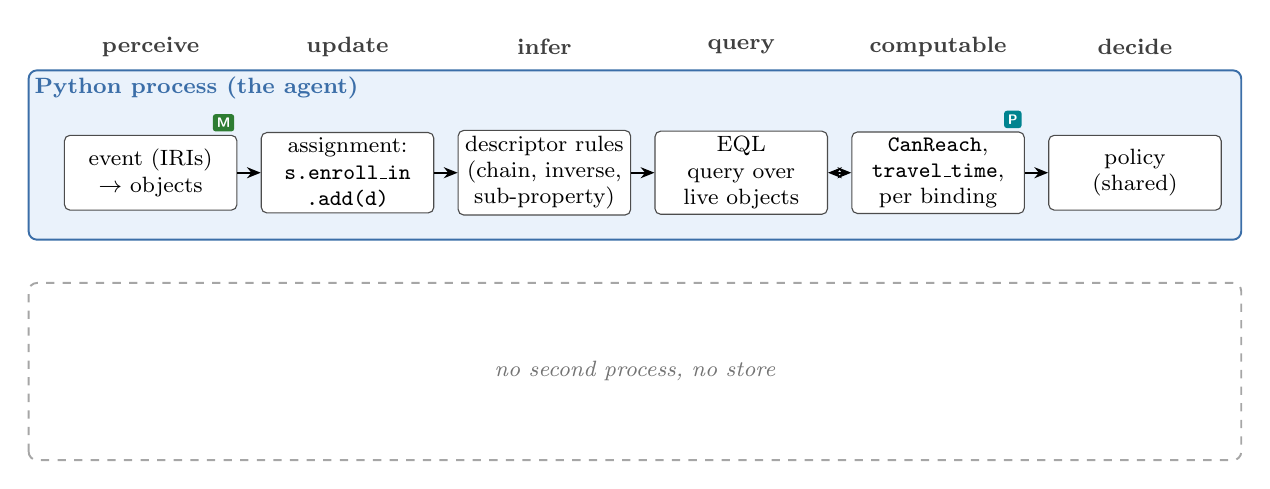
\begin{tikzpicture}
  \headers{perceive}{update}{infer}{query}{computable}{decide}
  \pylane{Python process (the agent)}
  \nolane{no second process, no store}
  \node[phasenode] (a) at (\cA,\yP) {event (IRIs)\\$\to$ objects};
  \node[phasenode] (b) at (\cB,\yP) {assignment:\\\texttt{s.enroll\textunderscore in}\\\texttt{.add(d)}};
  \node[phasenode] (c) at (\cC,\yP) {descriptor rules\\(chain, inverse,\\sub-property)};
  \node[phasenode] (d) at (\cD,\yP) {EQL query over\\live objects};
  \node[phasenode] (e) at (\cE,\yP) {\code{CanReach},\\\code{travel\_time},\\per binding};
  \node[phasenode] (f) at (\cF,\yP) {policy\\(shared)};
  \tagM{a} \tagP{e}
  \draw[flow] (a) -- (b); \draw[flow] (b) -- (c);
  \draw[flow] (c) -- (d);
  \draw[call] (d) -- (e);
  \draw[flow] (e) -- (f);
\end{tikzpicture}
\caption{KRROOD, one step. Everything runs in the agent's process on one world model: the inference happens in the
assignment, and the planner is called from inside the query. 0 round trips, 0 statements written elsewhere.}
\label{fig:krrood}
\end{figure}

% ---------------------------------------------------------------------
\subsection{GraphDB: a mirror in a server, the planner on the answers}
\label{sec:graphdb}

\paragraph{(a) Representation.} The application keeps its own objects: the robot, the campus map, and two lookups from
IRI to \code{Place} for course rooms and mail boxes. The OWL knowledge is a second world model: a GraphDB~11.2 repository
with the ruleset \code{owl2-rl-optimized}, into which setup loads the raw data; GraphDB materializes the closure during
the load (\file{graphdb\_variant.py}, class \code{GraphDBMirror}). The client keeps one HTTP connection open
(\code{requests.Session}) and passes the requested college as a SPARQL binding, so the query texts stay constant
(\file{rdf\_mirror.py}, \code{GraphDBSession}).

\paragraph{(b) Perception.} Every perceived fact is turned into RDF statements and sent in one \code{INSERT DATA} update
per step. An enrollment is two statements, the other events one each, so a step writes 3 to 6 statements.
\begin{lstlisting}[style=py]
@boundary(SYNCHRONIZATION)
def event_triples(event: KnowledgeEvent) -> List[Triple]:
    if isinstance(event, Enrollment):
        return [(event.person, RDF_TYPE, OWL2BENCH + "Person"),
                (event.person, OWL2BENCH + "enrollIn", event.department)]
    if isinstance(event, CourseTaking):
        return [(event.student, OWL2BENCH + "takesCourse", event.course)]
    if isinstance(event, CricketEnthusiasm):
        return [(event.person, OWL2BENCH + "isCrazyAbout", T20_CRICKET)]
    ...
@boundary(SYNCHRONIZATION)
def insert_data(triples: Iterable[Tuple[str, str, str]]) -> str:
    lines = [f"<{subject}> <{predicate}> {object_term(value)} ." for subject, predicate, value in triples]
    return "INSERT DATA {\n" + "\n".join(lines) + "\n}"

def perceive(self, perception: StepPerception, meter: StepMeter) -> None:
    with meter.phase("mapping"):
        triples = [triple for event in perception.knowledge_events for triple in event_triples(event)]
        update = insert_data(triples)
    with meter.phase("update"):
        self._send(update, meter)        # one HTTP request, counted as a round trip
    ...
\end{lstlisting}

\paragraph{(c) Inference.} GraphDB materializes the consequences of the inserted statements incrementally, inside the
update's transaction, before the request returns: \code{Student} from the domain of \code{enrollIn},
\code{isMemberOf} from the chain, \code{T20CricketFan} from the \code{hasValue} definition. The update's time therefore
includes the request, the commit and the inference.

\paragraph{(d) Computables.} SPARQL cannot call the robot's procedures. The query returns the IRIs that satisfy the
logical part; the build maps them back to the application's places and runs the planner in Python on the answers, once
per distinct room:
\begin{lstlisting}[style=py]
@boundary(MAPPING)
def _handout_rows(self, solutions: List[Dict[str, str]]) -> List[Tuple[str, str, Place]]:
    return [(s["student"], s["course"], self.course_rooms[s["course"]]) for s in solutions]

@boundary(PROCEDURE_INTEGRATION)
def _reachable_driving_times(self, rooms: set) -> Dict[Place, float]:
    return {room: travel_seconds(self.robot, room) for room in rooms if can_reach(self.robot, room)}
\end{lstlisting}

\paragraph{(e) Decision queries.} Two SPARQL queries per step, each one request (\code{?college} is bound per request):
\begin{lstlisting}[style=sq]
SELECT ?student ?course WHERE {
  ?student a owl2bench:Student ;
           owl2bench:isMemberOf ?college ;
           owl2bench:takesCourse ?course .
}
SELECT ?person WHERE {
  ?person a owl2bench:T20CricketFan .
}
\end{lstlisting}
\begin{lstlisting}[style=py]
def handout_candidates(self, college: str, meter: StepMeter) -> List[HandoutCandidate]:
    with meter.phase("query"):
        solutions = self._select(HANDOUT_QUERY, meter, college=college)
    with meter.phase("mapping"):
        rows = self._handout_rows(solutions)
    with meter.phase("query"):
        reachable = self._reachable_driving_times({room for _, _, room in rows})
        return [HandoutCandidate(student, course, room.identifier, reachable[room])
                for student, course, room in rows if room in reachable]
\end{lstlisting}
A step thus makes three requests: one update and two queries.

\begin{figure}[t]
\centering
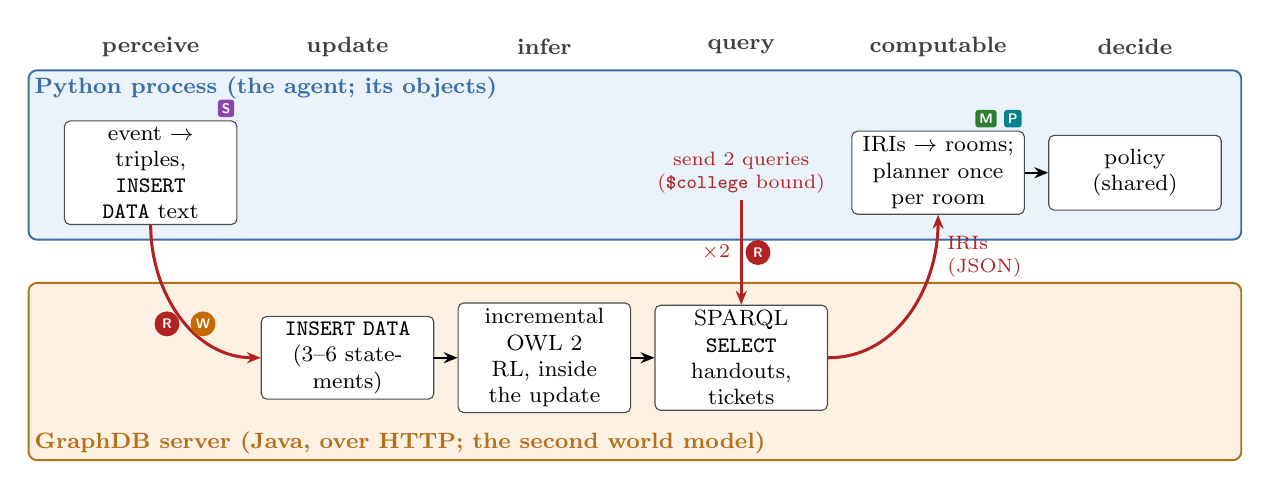
\begin{tikzpicture}
  \headers{perceive}{update}{infer}{query}{computable}{decide}
  \pylane{Python process (the agent; its objects)}
  \exlane{GraphDB server (Java, over HTTP; the second world model)}
  \node[phasenode] (a) at (\cA,\yP) {event $\to$ triples,\\\code{INSERT DATA} text};
  \node[phasenode] (b) at (\cB,\yX) {\code{INSERT DATA}\\(3--6 statements)};
  \node[phasenode] (c) at (\cC,\yX) {incremental\\OWL 2 RL, inside\\the update};
  \node[phasenode] (d) at (\cD,\yX) {SPARQL \code{SELECT}\\handouts, tickets};
  \node[phasenode] (e) at (\cE,\yP) {IRIs $\to$ rooms;\\planner once\\per room};
  \node[phasenode] (f) at (\cF,\yP) {policy\\(shared)};
  \coordinate (q) at (\cD,\yP);
  \node[font=\scriptsize, text=crossc, align=center] at (q) {send 2 queries\\(\code{\$college} bound)};
  \tagS{a} \tagMP{e}
  \draw[cross] (a.south) to[out=-90,in=180] node[pos=0.55, rt, xshift=-7pt] {R} node[pos=0.55, wr, xshift=6pt] {W} (b.west);
  \draw[flow] (b) -- (c); \draw[flow] (c) -- (d);
  \draw[cross] ([yshift=-10pt]q) -- node[rt, right=1pt] {R} node[left=2pt, crosslabel] {$\times$2} (d.north);
  \draw[cross] (d.east) to[out=0,in=-90] node[pos=0.8, crosslabel, right=3pt] {IRIs\\(JSON)} (e.south);
  \draw[flow] (e) -- (f);
\end{tikzpicture}
\caption{GraphDB, one step. Perception crosses into the server as an update (1 round trip, 3--6 statements), inference
runs there, the two queries cross over and back (2 round trips), and the planner runs in Python on the answers after
their IRIs are mapped back.}
\label{fig:graphdb}
\end{figure}

% ---------------------------------------------------------------------
\subsection{GraphDB, push: the planner's results written into the store}
\label{sec:push}

This build asks what it takes for SPARQL alone to decide (\file{graphdb\_push\_variant.py}). It shares the repository,
the loading and the mirroring of facts with the GraphDB build.

\paragraph{(a) Representation.} As in GraphDB, plus application data in the store under the prefix
\code{agent:} (namespace \url{https://example.org/agent-loop#}): at setup, \code{agent:taughtIn} for every course and \code{agent:mailbox} for
every person who exists at the start (\code{\_application\_triples}, 14 synchronization lines); every step, \code{agent:travelSeconds} for every
room the robot can reach now.

\paragraph{(b) Perception.} The first update of a step inserts the perceived facts and the mail box of each new person
(\code{\_knowledge\_triples}). A second update replaces the planner's results:
\begin{lstlisting}[style=py]
def perceive(self, perception: StepPerception, meter: StepMeter) -> None:
    with meter.phase("mapping"):
        triples = self._knowledge_triples(perception)
        update = insert_data(triples)
    with meter.phase("update"):
        self._send(update, meter)
    ...
    with meter.phase("push"):
        values = self._procedure_results()
        self._send(DELETE_PROCEDURE_RESULTS + " ;\n" + insert_data(values), meter)
    meter.statements_deleted += self.pushed_statements
    meter.statements_inserted += len(values)
\end{lstlisting}
\begin{lstlisting}[style=sq]
DELETE WHERE { ?room agent:travelSeconds ?seconds }
\end{lstlisting}

\paragraph{(c) Inference.} As in GraphDB: incremental OWL 2 RL inside each update. The pushed driving times are plain
data; no rule derives from them.

\paragraph{(d) Computables.} The planner runs \emph{before} the query, for every room a decision might need (the 201
course rooms and mail boxes of the scenario), because the store cannot ask for a value when it needs one. An unreachable
room gets no value, which encodes \code{can\_reach}:
\begin{lstlisting}[style=py]
@boundary(SYNCHRONIZATION)
def _procedure_results(self) -> List[Triple]:
    return [(place_iri(room.identifier), AGENT_LOOP + "travelSeconds",
             f'"{travel_seconds(self.robot, room)!r}"^^<{DOUBLE}>')
            for room in self.target_rooms if can_reach(self.robot, room)]
\end{lstlisting}
The robot moves almost every step, so nearly every value changes every step: about 200 statements are deleted and about
200 inserted.

\paragraph{(e) Decision queries.} One SPARQL query per decision selects, filters by reachability (a join with the pushed
values) and orders:
\begin{lstlisting}[style=sq]
SELECT ?student ?course ?room ?seconds WHERE {
  ?student a owl2bench:Student ;
           owl2bench:isMemberOf ?college ;
           owl2bench:takesCourse ?course .
  ?course agent:taughtIn ?room .
  ?room agent:travelSeconds ?seconds .
}
ORDER BY ?seconds ?course ?student

SELECT ?person ?room ?seconds WHERE {
  ?person a owl2bench:T20CricketFan ;
          agent:mailbox ?room .
  ?room agent:travelSeconds ?seconds .
}
ORDER BY ?seconds ?person
\end{lstlisting}
The answers are converted into candidate records (\code{\_handout\_records}, \code{\_ticket\_records} and
\code{place\_identifier}, mapping code). No procedure-integration code is left; its work moved into synchronization code.
A step makes four requests: two updates and two queries.

\begin{figure}[t]
\centering
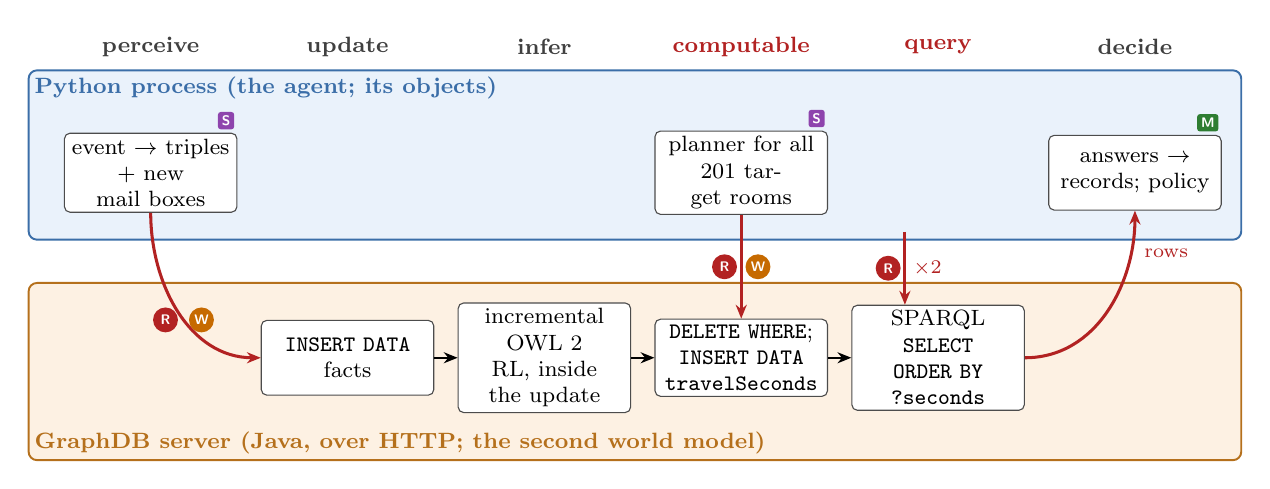
\begin{tikzpicture}
  \node[head] at (\cA,2.45) {perceive}; \node[head] at (\cB,2.45) {update}; \node[head] at (\cC,2.45) {infer};
  \node[headswap] at (\cD,2.45) {computable}; \node[headswap] at (\cE,2.45) {query}; \node[head] at (\cF,2.45) {decide};
  \pylane{Python process (the agent; its objects)}
  \exlane{GraphDB server (Java, over HTTP; the second world model)}
  \node[phasenode] (a) at (\cA,\yP) {event $\to$ triples\\+ new mail boxes};
  \node[phasenode] (b) at (\cB,\yX) {\code{INSERT DATA}\\facts};
  \node[phasenode] (c) at (\cC,\yX) {incremental\\OWL 2 RL, inside\\the update};
  \node[phasenode] (p) at (\cD,\yP) {planner for all\\201 target rooms};
  \node[phasenode] (s) at (\cD,\yX) {\code{DELETE WHERE};\\\code{INSERT DATA}\\\code{travelSeconds}};
  \node[phasenode] (d) at (\cE,\yX) {SPARQL \code{SELECT}\\\code{ORDER BY ?seconds}};
  \node[phasenode] (f) at (\cF,\yP) {answers $\to$\\records; policy};
  \tagS{a} \tagS{p} \tagM{f}
  \draw[cross] (a.south) to[out=-90,in=180] node[pos=0.55, rt, xshift=-7pt] {R} node[pos=0.55, wr, xshift=6pt] {W} (b.west);
  \draw[flow] (b) -- (c);
  \draw[flow] (c) -- (s);
  \draw[cross] (p.south) -- node[rt, left=1pt] {R} node[wr, right=1pt] {W} (s.north);
  \draw[flow] (s) -- (d);
  \draw[cross] ([xshift=-12pt]\cE,0.1) -- node[rt, left=1pt] {R} node[pos=0.5, crosslabel, right=1pt] {$\times$2} ([xshift=-12pt]d.north);
  \draw[cross] (d.east) to[out=0,in=-90] node[pos=0.8, crosslabel, right=3pt] {rows} (f.south);
\end{tikzpicture}
\caption{GraphDB with pushed planner results, one step. The planner runs before the query, for every room, and its
results cross into the store with the facts (2 updates, about 200 statements deleted and 200 inserted); then SPARQL
alone selects and orders (2 queries). 4 round trips.}
\label{fig:push}
\end{figure}

% ---------------------------------------------------------------------
\subsection{Nemo: a Datalog engine re-run every step}
\label{sec:nemo}

Nemo~0.10.1 materializes a program in one batch run of its command-line tool \code{nmo} and has no incremental mode
(\file{nemo\_variant.py}).

\paragraph{(a) Representation.} The application keeps its objects and IRI lookups, as in GraphDB. The OWL knowledge is
the raw OWL2Bench data (RDF/XML) plus an N-Triples file \file{perceived.nt} that holds every fact perceived so far.
The closure exists only during a run of \code{nmo}.

\paragraph{(b) Perception.} The step's facts are appended to the file, with the same \code{event\_triples} as the RDF
builds:
\begin{lstlisting}[style=py]
@boundary(SYNCHRONIZATION)
def _append_facts(self, perception: StepPerception) -> int:
    lines = [f"<{subject}> <{predicate}> {object_term(value)} .\n"
             for event in perception.knowledge_events
             for subject, predicate, value in event_triples(event)]
    with open(self.work_directory / "perceived.nt", "a") as stream:
        stream.writelines(lines)
    return len(lines)
\end{lstlisting}

\paragraph{(c) Inference.} Every step starts a new \code{nmo} process on one program: the OWL~2~RL/RDF rules
(\file{owl2rl.rls}, written for Nemo) with their import and export declarations replaced, so that both the raw data and
the perceived facts are input, and with the two decision rules added. Nemo computes the closure from scratch and exports
only the two decision predicates as CSV. According to the build's documentation, restarting from the previous step's
closure was slower in a trial, since Nemo treats every input fact as new.
\begin{lstlisting}[style=nm]
@parameter $input = "input.rdf" .
@parameter $perceived = "perceived.nt" .
@parameter $college = <http://benchmark/OWL2Bench#College> .
@import raw :- rdf{resource = $input} .
@import perceived :- ntriples{resource = $perceived} .
input(?s, ?p, ?o) :- raw(?s, ?p, ?o) .
input(?s, ?p, ?o) :- perceived(?s, ?p, ?o) .
...                                  % the OWL 2 RL/RDF rules
@export handout :- csv{resource = "handout.csv"} .
@export fan :- csv{resource = "fan.csv"} .
\end{lstlisting}

\paragraph{(d) Computables.} Nemo's rules cannot call the robot's procedures. As in GraphDB, the exported IRIs are
mapped to places and the planner runs in Python on the answers, once per distinct room
(\code{\_reachable\_driving\_times}, the same two lines).

\paragraph{(e) Decision queries.} The decisions are two rules over the closure predicate \code{triple/3} and its view
\code{rdf\_type/2}; the requested college is the parameter \code{\$college}, passed on the command line:
\begin{lstlisting}[style=nm]
handout(?student, ?course) :- rdf_type(?student, owl2bench:Student),
    triple(?student, owl2bench:isMemberOf, $college), triple(?student, owl2bench:takesCourse, ?course) .
fan(?person) :- rdf_type(?person, owl2bench:T20CricketFan) .
\end{lstlisting}
\begin{lstlisting}[style=py]
command = [self.nemo_binary, "--overwrite-results", "--export-dir", str(export_directory), "--report", "short",
           "--param", f'input="{Path(UNREASONED_FILE).resolve()}"',
           "--param", f'perceived="{self.work_directory / "perceived.nt"}"',
           "--param", f"college=<{college}>",
           str(self.work_directory / "step.rls")]
completed = subprocess.run(command, capture_output=True, text=True, check=True)
\end{lstlisting}
The run happens in \code{perceive} (phase ``reasoning''); the two decision methods only read the stored answers. A step
makes no server request; it starts one process and reads two files.

\begin{figure}[t]
\centering
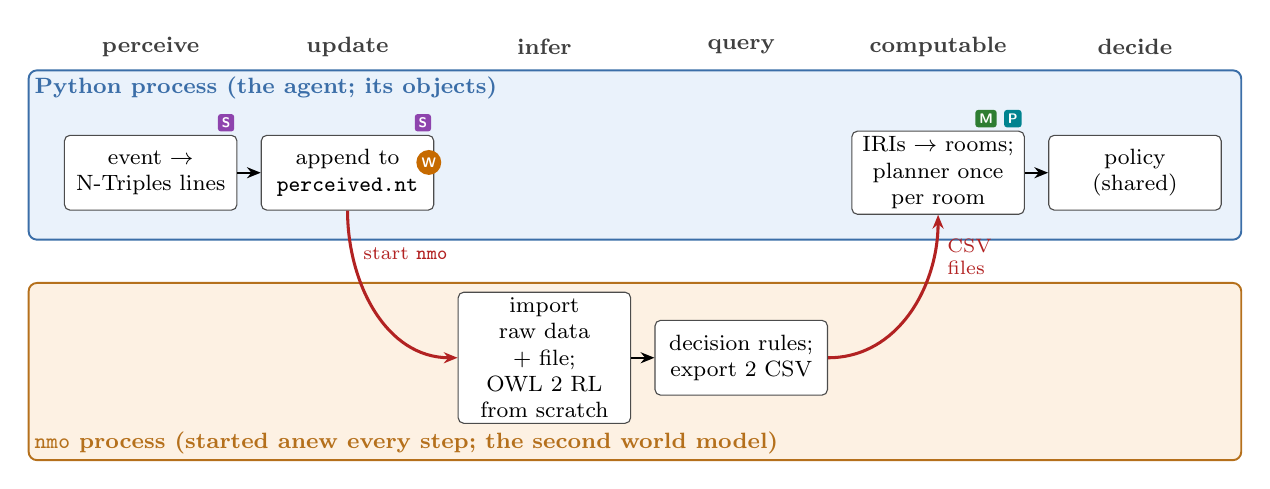
\begin{tikzpicture}
  \headers{perceive}{update}{infer}{query}{computable}{decide}
  \pylane{Python process (the agent; its objects)}
  \exlane{\code{nmo} process (started anew every step; the second world model)}
  \node[phasenode] (a) at (\cA,\yP) {event $\to$\\N-Triples lines};
  \node[phasenode] (b) at (\cB,\yP) {append to\\\file{perceived.nt}};
  \node[phasenode] (c) at (\cC,\yX) {import raw data\\+ file; OWL 2 RL\\from scratch};
  \node[phasenode] (d) at (\cD,\yX) {decision rules;\\export 2 CSV};
  \node[phasenode] (e) at (\cE,\yP) {IRIs $\to$ rooms;\\planner once\\per room};
  \node[phasenode] (f) at (\cF,\yP) {policy\\(shared)};
  \tagS{a} \tagS{b} \tagMP{e}
  \draw[flow] (a) -- (b);
  \node[wr] at ($(b.north east)+(-2pt,-10pt)$) {W};
  \draw[cross] (b.south) to[out=-90,in=180] node[pos=0.2, crosslabel, right=2pt] {start \code{nmo}} (c.west);
  \draw[flow] (c) -- (d);
  \draw[cross] (d.east) to[out=0,in=-90] node[pos=0.8, crosslabel, right=3pt] {CSV\\files} (e.south);
  \draw[flow] (e) -- (f);
\end{tikzpicture}
\caption{Nemo, one step. Perception appends to a file (about 4 statements); a new process recomputes the whole closure
and the two decision rules; the planner runs in Python on the exported answers. No server request; one process start
per step.}
\label{fig:nemo}
\end{figure}

% ---------------------------------------------------------------------
\subsection{Owlready2: Pellet re-run every step}
\label{sec:owlready2}

Owlready2~0.49 keeps OWL individuals in a quadstore (SQLite) inside the Python process and exposes them as Python
objects; inference is Pellet's, which Owlready2 runs as a Java process (\file{owlready2\_variant.py}).

\paragraph{(a) Representation.} The knowledge is Owlready2's quadstore, read and written through its Python objects,
which are proxies of the stored individuals. The application keeps its rooms and mail boxes in dictionaries by IRI, as
in GraphDB, because Owlready2 may discard a proxy and re-create it from the store, losing attributes set on it.

\paragraph{(b) Perception.} A perceived fact is an assignment on Owlready2's objects, which writes the asserted
statement into the quadstore and infers nothing. Events name individuals by IRI, which the build resolves with
\code{world[iri]} (mapping, as KRROOD resolves IRIs to its objects):
\begin{lstlisting}[style=py]
department = self._individual(event.department)              # world[iri]
person = self._new_individual(event.person, OWL2BENCH + "Person")
self.world[OWL2BENCH + "enrollIn"][person].append(department)
\end{lstlisting}

\paragraph{(c) Inference.} After the step's facts, the build deletes the previous step's inferences and runs Pellet
again with \code{infer\_property\_values=True}. Owlready2 exports the whole world to Pellet and writes Pellet's
inferences back, about 1.36 million statements, into an ontology of their own:
\begin{lstlisting}[style=py]
@boundary(SYNCHRONIZATION)
def _delete_inferences(self) -> None:
    if self.inferred is not None:
        self.inferred.destroy()

@boundary(SYNCHRONIZATION)
def _run_pellet(self) -> None:
    self.inferred = self.world.get_ontology(INFERRED_ONTOLOGY.format(self.pellet_runs))
    self.pellet_runs += 1
    with self.inferred:
        owlready2.sync_reasoner_pellet(self.world, infer_property_values=True, debug=0)
\end{lstlisting}
Keeping the previous inferences instead would make Pellet read the whole closure every step, which takes about
19 minutes and a 22\,GB heap (the loading benchmark's pre-reasoned input). Pellet's model exists only during its run,
like Nemo's closure; it is the second world model.

\paragraph{(d) Computables.} Pellet cannot call the robot's procedures. The answers' IRIs are mapped to places and the
planner runs in Python on them, once per distinct room, with the same two lines as GraphDB and Nemo.

\paragraph{(e) Decision queries.} The decisions use Owlready2's Python API, so the developer writes Python only:
\begin{lstlisting}[style=py]
students = self.world.search(type=self.world[OWL2BENCH + "Student"], isMemberOf=college)
pairs = [(student, course) for student in students
         for course in self.world[OWL2BENCH + "takesCourse"][student]]
fans = list(self.world.search(type=self.world[OWL2BENCH + "T20CricketFan"]))
\end{lstlisting}
A step makes no server request; it starts one Java process.

\begin{figure}[t]
\centering
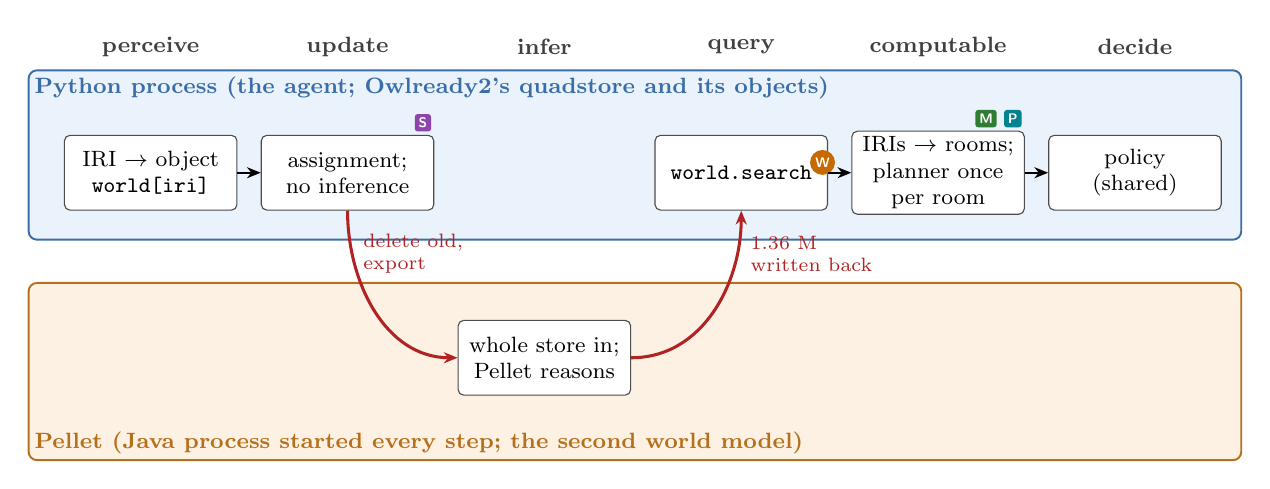
\begin{tikzpicture}
  \headers{perceive}{update}{infer}{query}{computable}{decide}
  \pylane{Python process (the agent; Owlready2's quadstore and its objects)}
  \exlane{Pellet (Java process started every step; the second world model)}
  \node[phasenode] (a) at (\cA,\yP) {IRI $\to$ object\\\code{world[iri]}};
  \node[phasenode] (b) at (\cB,\yP) {assignment;\\no inference};
  \node[phasenode] (c) at (\cC,\yX) {whole store in;\\Pellet reasons};
  \node[phasenode] (d) at (\cD,\yP) {\code{world.search}};
  \node[phasenode] (e) at (\cE,\yP) {IRIs $\to$ rooms;\\planner once\\per room};
  \node[phasenode] (f) at (\cF,\yP) {policy\\(shared)};
  \tagS{b} \tagMP{e}
  \draw[flow] (a) -- (b);
  \draw[cross] (b.south) to[out=-90,in=180] node[pos=0.2, crosslabel, right=2pt] {delete old,\\export} (c.west);
  \draw[cross] (c.east) to[out=0,in=-90] node[pos=0.8, crosslabel, right=3pt] {1.36 M\\written back} (d.south);
  \node[wr] at ($(d.north east)+(-2pt,-10pt)$) {W};
  \draw[flow] (d) -- (e); \draw[flow] (e) -- (f);
\end{tikzpicture}
\caption{Owlready2, one step. Perception asserts on Owlready2's objects; the previous inferences are deleted, Pellet
reasons on the exported store, and its inferences are written back; the planner runs in Python on the answers of a
search. No server request; one process start per step.}
\label{fig:owlready2}
\end{figure}

% ---------------------------------------------------------------------
\subsection{reasonable (briefly)}
\label{sec:reasonable}

reasonable~0.4.4 is an in-memory OWL~2~RL reasoner written in Rust with Python bindings (\file{reasonable\_variant.py}).
Setup parses the raw data with RDFLib and materializes the closure. Every step adds the perceived facts as RDFLib
statements with \code{from\_graph} and calls \code{reason()}. reasonable materializes additions incrementally, but
\code{reason()} returns the whole closure as a list of RDFLib triples, so the step includes building that list. The
build then makes one pass over the returned triples (\code{ClosureIndex.of}) to collect students, fans, members and
courses, maps the answers to places, and runs the planner on them, as GraphDB does. It runs in one process, but the
closure is a second world model in another data structure, written in another language. reasonable~0.4.4 does not
implement the property-chain rule \code{prp-spo2}, so it never infers \code{isMemberOf} of a college and finds no
handout candidates. This is recorded, not repaired. It was run for seed~0 only, as it needs about 17\,GB.

\begin{figure}[t]
\centering
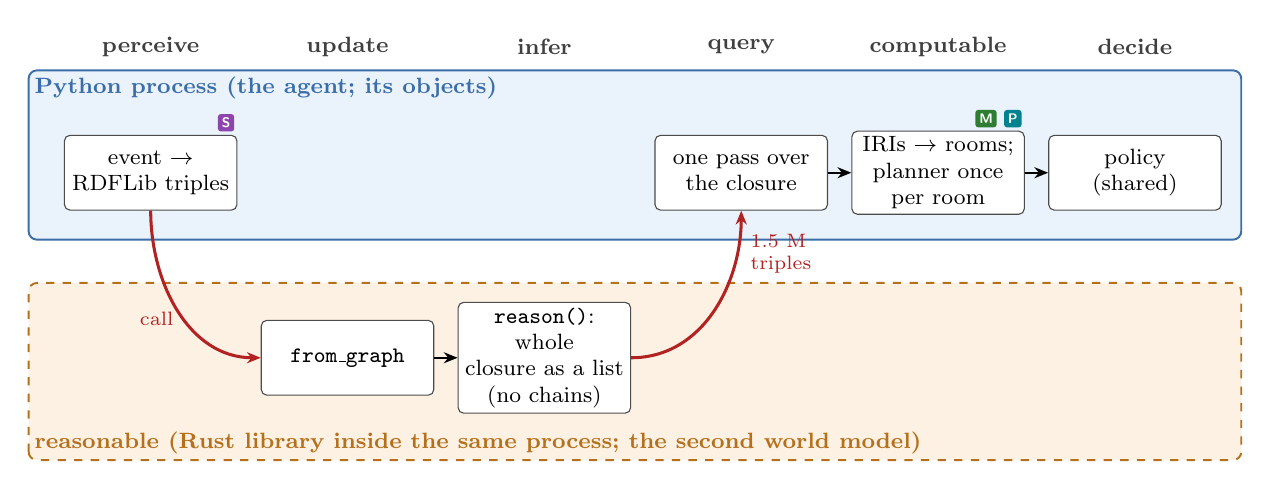
\begin{tikzpicture}
  \headers{perceive}{update}{infer}{query}{computable}{decide}
  \pylane{Python process (the agent; its objects)}
  \exlane[dashed]{reasonable (Rust library inside the same process; the second world model)}
  \node[phasenode] (a) at (\cA,\yP) {event $\to$\\RDFLib triples};
  \node[phasenode] (b) at (\cB,\yX) {\code{from\_graph}};
  \node[phasenode] (c) at (\cC,\yX) {\code{reason()}: whole\\closure as a list\\(no chains)};
  \node[phasenode] (d) at (\cD,\yP) {one pass over\\the closure};
  \node[phasenode] (e) at (\cE,\yP) {IRIs $\to$ rooms;\\planner once\\per room};
  \node[phasenode] (f) at (\cF,\yP) {policy\\(shared)};
  \tagS{a} \tagMP{e}
  \draw[cross] (a.south) to[out=-90,in=180] node[pos=0.55, crosslabel, left=2pt] {call} (b.west);
  \draw[flow] (b) -- (c);
  \draw[cross] (c.east) to[out=0,in=-90] node[pos=0.8, crosslabel, right=3pt] {1.5 M\\triples} (d.south);
  \draw[flow] (d) -- (e); \draw[flow] (e) -- (f);
\end{tikzpicture}
\caption{reasonable, one step. Two calls into the native library (no server request); the whole closure comes back
every step and is scanned in Python.}
\label{fig:reasonable}
\end{figure}

% =====================================================================
\section{How the rows of Table 4 are measured}
\label{sec:measure}

Table~4 groups its rows by what they follow from. The upper rows follow from evaluating EQL queries over the program's
objects: a build of this kind has one world model, calls the planner in the query and writes nothing to another store.
The lower rows follow from the implementation: one language and one process could also come from a wrapper that
generates SPARQL or from an embedded store, which would still keep two world models. Owlready2 shows the first: its
build is written only in Python and still keeps a second world model, Pellet's.

\subsection{Rows from the semantics}

\paragraph{World models.} The number of representations of the robot's world knowledge that the build keeps up to date:
the objects (always), plus the GraphDB repository (both GraphDB builds), the input files and Nemo's closure (Nemo),
reasonable's closure, or Pellet's model, rebuilt every step from Owlready2's quadstore (Owlready2). For Owlready2 the
objects and the quadstore count as one, as the objects are proxies of the stored individuals. Read from the code.

\paragraph{Planner vs.\ query.} Where \code{can\_reach} and \code{travel\_seconds} are evaluated relative to the logical
query. \emph{Inside}: as an EQL predicate and symbolic function, per binding, on the live robot. \emph{After}: in Python,
after the query, once per distinct room among the answers (GraphDB, Nemo, Owlready2, reasonable). \emph{Before}: for every
room a decision could need, with the results written into the store (GraphDB push). The \code{ProcedureMeter} counts the
calls. For seed~0, the mean number of \code{can\_reach} calls per step is 1,310.7 for KRROOD (per binding), 59.5 for
GraphDB (per distinct room among the answers) and 201 for GraphDB push (every target room)
(\file{agent\_loop.json}).

\paragraph{Writes.} Statements written in a step because of the second world model, inserted plus deleted, as counted
by the build in \code{StepMeter.statements\_inserted} and \code{statements\_deleted}: the statements of the
\code{INSERT DATA} updates (GraphDB), plus the deleted and inserted \code{travelSeconds} values (push), the lines
appended to \file{perceived.nt} (Nemo), or the previous step's inferences deleted and Pellet's inferences written back,
with the step's asserted facts (Owlready2; medians 1,358,555 deleted and 1,358,558 inserted, 2.7 million in all). The
median over the 1,000 steps of the five seeds is reported, for Owlready2 over its 200 steps of seed~0. KRROOD has no second
world model, so the table reports 0. Its meter does count its descriptor assignments in \code{statements\_inserted}
(median 5 per step: three per enrollment, counting the new person and the mail box, and one per other event), but these
are the update itself, not a copy of it.

\paragraph{Sync.\ lines.} Lines of code that exist only to keep the second representation in agreement with the
application's facts, counted as in Section~\ref{sec:lines}. For Owlready2 these are the two functions that delete the
previous inferences and run Pellet.

\subsection{Rows from the implementation}

\paragraph{Languages.} The languages in which the developer writes the decision: Python (KRROOD); Python and SPARQL
(both GraphDB builds); Python and Nemo's rule language (Nemo); Python (Owlready2, through its search API).

\paragraph{Processes.} The operating-system processes that hold or compute the robot's knowledge: the Python worker
(KRROOD, reasonable); the worker and the GraphDB server, a Java process reached over HTTP (GraphDB builds); the worker
and one \code{nmo} process started per step (Nemo); the worker and one Java process for Pellet started per step
(Owlready2).

\paragraph{Round trips per step.} Requests to a server in a step. \code{GraphDBMirror.\_send} (updates) and
\code{\_select} (queries) increment \code{StepMeter.round\_trips} once per HTTP request. The count is constant: 3 for
GraphDB (one update, two queries) and 4 for push (two updates, two queries). KRROOD, Nemo, Owlready2 and reasonable make no server
requests; Nemo's and Pellet's process start and reasonable's two library calls per step are counted separately as
\code{reasoner\_calls} (1, 1 and 2); Table~4 shows a process start as ``1 run''.

\paragraph{Step [ms].} The wall time of a step, from \code{StepMeter} (\file{measurement.py}). The loop
(\file{loop.py}, \code{run\_agent\_loop}) times every part of a step as a phase with \code{time.perf\_counter}:
\begin{itemize}
  \item \code{mapping}: translating between the objects and another representation;
  \item \code{update}: writing the perceived facts, including the inference that happens on insertion (descriptor
        chaining in KRROOD, GraphDB's incremental materialization inside the update request);
  \item \code{reasoning}: a separate materialization call (Nemo's run, reasonable's \code{reason()}, Owlready2's deletion
        of the previous inferences and Pellet's run);
  \item \code{push}: writing the planner's results into the store (push only);
  \item \code{query}: evaluating the decision queries, without the time inside the procedures;
  \item \code{procedures}: the time inside \code{can\_reach} and \code{travel\_seconds}, wherever they are called
        from. The \code{ProcedureMeter} times every call, and the enclosing phase's time is reduced by it;
  \item \code{decide} and \code{act}: the shared policy and the robot's motion.
\end{itemize}
The step time is the sum of the phases. It excludes setup (loading and materializing the closure) and the bookkeeping of
the experiment (the digest of the candidates). The table reports the median over the 1,000 steps of the five seeds (for Owlready2, over its 200 steps of seed~0);
every seed's median lies within 7.4\% of it; the results file also holds a 95\% bootstrap interval of the
median and the 95th percentile (\file{agent\_loop\_seeds.json}).

\paragraph{Agreement.} Not a row, but the precondition for comparing the rows. For every step, the build's own action
and its candidate sets (sorted, de-duplicated, driving times rounded to microseconds, hashed) are compared with the
reference's.

\subsection{The line count}
\label{sec:lines}

\paragraph{The line count.} Code is attributed by marking functions with the decorator
\code{@boundary(category)} of \file{measurement.py}. There are three categories:
\begin{itemize}
  \item \code{SYNCHRONIZATION}: code that writes the application's facts into a second representation;
  \item \code{MAPPING}: code that translates between the application's objects and another representation (IRIs to
        objects, objects to IRIs, query results to application records);
  \item \code{PROCEDURE\_INTEGRATION}: code that makes the robot's procedures usable in a decision, either a predicate
        class or symbolic function that wraps a procedure, or the Python filter applied to the answers of a query that
        cannot call it.
\end{itemize}
\code{boundary\_functions} collects the marked methods of the build's class and its base classes (the most derived
definition of each name) and the module-level functions the class lists in \code{boundary\_helpers} (for example the
shared \code{event\_triples}, \code{insert\_data} and \code{object\_term} of \file{rdf\_mirror.py}).
\code{code\_lines} counts the lines of each function's source that hold code: it drops blank lines, comment lines,
decorator lines and every string-literal statement (function and attribute docstrings). The \code{def} or \code{class}
line counts. Table~\ref{tab:lines} lists the counted functions. The bodies of \code{perceive},
\code{handout\_candidates} and \code{ticket\_candidates} are not marked in any build; they are the step's control flow,
which every build has.

\begin{table}[t]
\centering
\caption{The marked functions and their code lines, from the \code{boundary\_lines} entries of the results files.}
\label{tab:lines}
\footnotesize
\begin{tabular}{@{}llr@{\hspace{2em}}llr@{}}
\toprule
\multicolumn{3}{@{}l}{\textbf{KRROOD} (0 / 12 / 7)} & \multicolumn{3}{l@{}}{\textbf{GraphDB} (16 / 9 / 2)}\\
\midrule
\code{\_attach\_application\_data} & M & 8 & \code{event\_triples} & S & 11\\
\code{\_resolve} & M & 2 & \code{insert\_data} & S & 3\\
\code{\_register} & M & 2 & \code{object\_term} & S & 2\\
\code{CanReach} & P & 5 & \code{\_application\_data} & M & 4\\
\code{travel\_time} & P & 2 & \code{\_handout\_rows}, \code{\_ticket\_rows} & M & 2, 3\\
 & & & \code{\_reachable\_driving\_times} & P & 2\\
\midrule
\multicolumn{3}{@{}l}{\textbf{GraphDB, push} (44 / 15 / 0)} & \multicolumn{3}{l@{}}{\textbf{Nemo} (22 / 9 / 2)}\\
\midrule
\code{\_application\_triples} & S & 14 & \code{\_append\_facts} & S & 9\\
\code{\_knowledge\_triples} & S & 8 & \code{event\_triples} & S & 11\\
\code{\_procedure\_results} & S & 6 & \code{object\_term} & S & 2\\
\code{event\_triples}, \code{insert\_data}, \code{object\_term} & S & 11, 3, 2 & \code{\_application\_data} & M & 4\\
\code{\_application\_data} & M & 4 & \code{\_handout\_rows}, \code{\_ticket\_rows} & M & 2, 3\\
\code{\_handout\_records}, \code{\_ticket\_records} & M & 5, 2 & \code{\_reachable\_driving\_times} & P & 2\\
\code{place\_iri}, \code{place\_identifier} & M & 2, 2 & & & \\
\midrule
\multicolumn{3}{@{}l}{\textbf{Owlready2} (8 / 15 / 2)} & & & \\
\midrule
\code{\_delete\_inferences} & S & 3 & \code{\_application\_data} & M & 4\\
\code{\_run\_pellet} & S & 5 & \code{\_individual}, \code{\_new\_individual} & M & 2, 4\\
\code{\_reachable\_driving\_times} & P & 2 & \code{\_handout\_rows}, \code{\_ticket\_rows} & M & 2, 3\\
\bottomrule
\end{tabular}
\end{table}

\paragraph{Mapping and procedure lines: in the total only.} The line count also attributes lines of code that
translate between the application's objects and another representation (mapping) and lines that make the robot's
procedures usable in a decision (procedure integration). The results files hold them (\code{boundary\_lines}, per
category; Table~\ref{tab:lines}), and the supplement's report lists them. The paper's Table~4 shows them only within
the total, ``Boundary lines'', as they do not measure a second world model. The mapping lines follow from the simulated perceptions, which
arrive as IRIs in every build: KRROOD, with one world model, also resolves them to objects (12 lines). The procedure
lines follow from wrapping the planner, as a predicate and a function in KRROOD (7 lines) or as a filter of the
answers in GraphDB and Nemo (2 lines), not from the number of world models.

% =====================================================================
\section{Results}
\label{sec:results}

\paragraph{Runs.} The numbers of Table~4 come from the measured run of the supplement's results
(\file{results/agent\_loop/}): seeds 0--4, 200 steps each, three perceived facts per step, one run per build and
seed, on an Intel Core i7-13700 with 64\,GB RAM under Ubuntu 24.04, in a Docker container pinned to six cores, with
GraphDB~11.2 Free (one core, 6\,GB heap) in the same container (\file{provenance.txt}). Nemo was run separately, five seeds
of 200 steps on other cores, with KRROOD alongside as the reference of the agreement check. Owlready2 was run last,
seed~0 with 200 steps, in the same image pinned to the same six cores, with KRROOD alongside as the reference and
nothing else running (\file{results/agent\_loop\_owlready2/provenance.txt}).

\paragraph{The table.} The paper's Table~4 reads (push: GraphDB with the planner's results written into the store):
\begin{center}
\footnotesize
\begin{tabular}{@{}lrrrrr@{}}
\toprule
 & \textbf{KRROOD} & \textbf{GraphDB} & \textbf{push} & \textbf{Nemo} & \textbf{Owlready2}\\
\midrule
\multicolumn{6}{@{}l}{\emph{From the semantics}}\\
World models & 1 & 2 & 2 & 2 & 2\\
Planner vs.\ query & inside & after & before & after & after\\
Writes & 0 & 4 & 405 & 4 & 2.7\,M\\
Sync.\ lines & 0 & 16 & 44 & 22 & 8\\
\multicolumn{6}{@{}l}{\emph{From the implementation}}\\
Languages & 1 & 2 & 2 & 2 & 1\\
Processes & 1 & 2 & 2 & 2 & 2\\
Round trips & 0 & 3 & 4 & 1 run & 1 run\\
Boundary lines & 19 & 27 & 59 & 33 & 25\\
Step [ms] & 90 & 96 & 162 & 5{,}683 & 32{,}986\\
\bottomrule
\end{tabular}
\end{center}
The seeds' median steps range over 88--90 (KRROOD), 93--100 (GraphDB), 150--166 (push) and 5,653--5,690\,ms (Nemo).
GraphDB push writes 405 statements per step: 204 inserted and 201 deleted (medians).

\paragraph{What the rows show.}
\begin{itemize}
  \item \emph{One world model is enough.} KRROOD decides with no synchronization code, no writes to another store and
        no requests. Outside the table, its 12 mapping lines resolve the IRIs in which events name individuals and
        attach the application data, and its 7 procedure lines are the predicate and the function
        (Section~\ref{sec:lines}).
  \item \emph{A second world model costs code and traffic.} GraphDB needs 16 lines to mirror facts and three requests
        per step; outside the table, 9 more lines map answers back and 2 filter them with the planner.
  \item \emph{Letting the store decide moves the planner out of the decision.} With the planner's results pushed, SPARQL
        decides alone and the procedure lines drop to 0, but the synchronization lines grow to 44, the writes to about
        400 statements per step, and the planner runs for every room in every step, whether a decision needs it or
        not.
  \item \emph{Step times are comparable, but spent differently.} The median phases (\file{agent\_loop\_seeds.json})
        are: KRROOD, 88.3\,ms in queries and 0.43\,ms in the update; GraphDB, 88.9\,ms in the update and 7.5\,ms in
        queries; push, 87.2\,ms in the update, 63.0\,ms in the push and 15.5\,ms in queries. A GraphDB update costs
        about 38\,ms even when empty (median of 30 empty updates, \file{graphdb\_update\_cost.json}). The navigation
        form of KRROOD's handout query brings KRROOD's median step to 74\,ms.
  \item \emph{Recomputing the closure every step is slow.} Nemo makes the same decisions with a median step of 5.68\,s
        (seeds' medians 5.65--5.69\,s), nearly all of it Nemo's run (by its own report, about 2.2\,s import and 3.4\,s
        reasoning). In the table, Nemo has 2 world models, runs the planner on the answers, appends a median of 4
        statements per step, has 22 synchronization lines, uses 2 languages and 2 processes, and makes no server
        request but starts one process per step (``1 run''); outside the table, it has 9 mapping and 2 procedure
        lines. reasonable takes 4.6\,s per step
        (seed~0) and finds no handout candidate.
  \item \emph{One language does not remove the second world model.} Owlready2's build is written only in Python and
        makes the same decisions, but every step it deletes the previous step's 1.36 million inferences, Owlready2
        exports the quadstore to Pellet, and Pellet's 1.36 million inferences are written back: a median step of
        33.0\,s (95th percentile 34.0\,s), about 2\,s deleting and 31\,s in Pellet's run, with 8 synchronization
        lines. Keeping the inferences instead would make Pellet read the whole closure every step, about 19 minutes on
        the loading benchmark's pre-reasoned input.
\end{itemize}

\paragraph{Agreement.} Both GraphDB builds and Nemo make KRROOD's decision and return KRROOD's candidate sets in all
1,000 steps. For Nemo the candidate files of both are identical in every seed. Owlready2 makes KRROOD's decision and returns its candidate sets in all 200 steps of seed~0;
its candidate file is identical to KRROOD's. reasonable agrees on the action in 104
of 200 steps and on the candidate sets in 2, because it derives no property chains.

\end{document}
